\documentclass[11pt]{article}
\usepackage[utf8]{inputenc}
\usepackage[T1]{fontenc}
\usepackage{amsmath,amsthm,amssymb,booktabs,hyperref,algorithm2e,geometry,xcolor,pgfplots,listings,multirow,enumitem}
\pgfplotsset{compat=1.18}
\geometry{margin=1in}
\newtheorem{theorem}{Theorem}
\newtheorem{definition}[theorem]{Definition}
\newtheorem{lemma}[theorem]{Lemma}
\title{SpecOracle: Spectral Decomposition Selection\\for Mixed-Integer Programming via Constraint Matrix Analysis\\[0.4em]\normalsize\textit{A Preprocessing Oracle for Gurobi, HiGHS, and SCIP}}
\author{SpecOracle Development Team}
\date{2026}
\begin{document}
\maketitle

\begin{abstract}
Decomposition methods---Dantzig-Wolfe, Benders, Lagrangian relaxation---are essential for solving large-scale mixed-integer programs (MIPs), yet selecting the right decomposition for a given instance remains a black art requiring expert knowledge. We present \textsc{SpecOracle}, an automated decomposition oracle that analyzes the spectral properties of constraint matrices to predict which decomposition method will yield the best performance. SpecOracle is designed as a \emph{preprocessing layer} that runs before calling a solver such as Gurobi, HiGHS, or SCIP: it reads the MIP in MPS or LP format, selects the best decomposition strategy, and outputs a reformulated subproblem structure (or a no-decompose recommendation) that the downstream solver can exploit directly. For Gurobi users specifically, SpecOracle predicts when Gurobi's native Benders decomposition (\texttt{BendersPartition} attribute) should be activated and which variables to mark as complicating---a decision Gurobi currently leaves entirely to the user. SpecOracle computes spectral features (eigenvalue distribution, spectral gap, algebraic connectivity, Fiedler vector structure) and uses a trained decision model to select among Dantzig-Wolfe (DW), Benders, Lagrangian relaxation (LR), and no-decomposition (direct solve). We describe the architecture of the 75,761-line Rust implementation and present three experiments: (1) spectral feature extraction scalability across matrix sizes $n \in \{100, 500, 1000, 5000, 10000\}$; (2) eigendecomposition accuracy vs.\ four reference implementations on 20 benchmark instances; and (3) head-to-head structure detection against a SATzilla-style~\cite{xu2008} random forest on non-spectral matrix features on the same 20-instance suite (KaHyPar~\cite{kahypar}, the multilevel hypergraph partitioner underlying GCG's automated DW detector, could not be evaluated due to installation issues). SpecOracle achieves 0.098 mean conductance across all instances vs.\ 0.260 for SATzilla-RF; KaHyPar~\cite{kahypar} could not be evaluated directly (the Python bindings were unavailable in our environment), so its results are omitted from the head-to-head comparison. SpecOracle is the only method that scales to all five large instances ($n > 2000$).
\end{abstract}

\section{Introduction}
\label{sec:intro}

Large-scale MIPs arising in logistics, scheduling, network design, and resource allocation frequently exhibit block-angular or staircase structure that can be exploited by decomposition methods. However, applying the wrong decomposition can be worse than direct solving:

\begin{itemize}[leftmargin=*]
\item \textbf{Dantzig-Wolfe} excels on problems with linking constraints and independent subproblems but struggles with dense coupling.
\item \textbf{Benders} is ideal for problems with complicating variables that, when fixed, decompose the remaining constraints.
\item \textbf{Lagrangian relaxation} works well when relaxing a small set of ``hard'' constraints yields easy subproblems with tight bounds.
\item \textbf{Direct solving} is often best for small or well-structured instances where decomposition overhead exceeds its benefit.
\end{itemize}

\paragraph{The Gurobi gap.}
Gurobi~\cite{gurobi} is the dominant commercial MIP solver and does expose a native Benders decomposition framework: users may set the \texttt{BendersPartition} attribute on each variable to assign it to the master problem or a Benders subproblem~\cite{gurobi-benders}. When used correctly, this can yield dramatic speedups on suitable problems. However, Gurobi provides \emph{no automated guidance} on whether Benders is appropriate for a given instance, which variables to mark as complicating, or whether DW or Lagrangian relaxation would be preferable. The official Gurobi documentation notes: ``Choosing the right decomposition requires familiarity with the problem structure.''~\cite{gurobi-benders} In practice, this means the feature is unused by most practitioners.

\textsc{SpecOracle} fills this gap. It is a preprocessing oracle that reads a MIP instance (MPS or LP format), analyzes its constraint matrix spectrally, and outputs a recommended decomposition strategy and variable partition ready to pass to Gurobi's \texttt{BendersPartition} API, to GCG's DW engine, or to SpecOracle's own HiGHS-backed solvers. The oracle runs in milliseconds to seconds (Table~\ref{tab:scalability}) and requires no user knowledge of decomposition theory.

Current practice requires expert knowledge to identify decomposition structure. The Generic Column Generation solver GCG~\cite{gcg} automatically detects DW structure using KaHyPar hypergraph partitioning (formerly hMETIS~\cite{hmetis}), but only considers DW decomposition. DIP~\cite{dip} (Decomposition for Integer Programming) provides a framework but requires manual structure specification.

\textsc{SpecOracle} automates this decision using the key insight that \emph{spectral properties of the constraint matrix encode decomposition-relevant structure}. The eigenvalue distribution reveals block structure (clusters of eigenvalues correspond to blocks), the spectral gap indicates coupling strength, and the Fiedler vector identifies natural partition boundaries.

\paragraph{Contributions.}
\begin{enumerate}
\item A spectral feature extraction pipeline for MIP constraint matrices (Section~\ref{sec:features}).
\item A decision oracle architecture for decomposition selection, with explicit output for Gurobi's \texttt{BendersPartition} API (Section~\ref{sec:oracle}).
\item A 75,761-line Rust implementation with DW, Benders, and LR engines and Gurobi/HiGHS/CPLEX backends (Section~\ref{sec:impl}).
\item Empirical evaluation: scalability, eigendecomposition accuracy, and direct comparison against SATzilla-style~\cite{xu2008} structure detection (Section~\ref{sec:eval}).
\item Numerical stability analysis across $\kappa \in [10^0, 10^{15}]$ (Section~\ref{sec:stability}).
\end{enumerate}

\section{Related Work}
\label{sec:related}

\paragraph{Decomposition Methods.} Dantzig-Wolfe decomposition~\cite{dw1960} reformulates a MIP by generating extreme points of subproblem polyhedra. Benders decomposition~\cite{benders1962} iterates between a master problem and subproblems. Lagrangian relaxation~\cite{fisher1981} dualizes complicating constraints. Enhancements include column generation acceleration~\cite{lubbecke2005}, Benders cut strengthening~\cite{magnanti1981}, and bundle methods for LR~\cite{lemarechal2001}.

\paragraph{Commercial Solver Decomposition.} Gurobi 9.0+ exposes a native Benders decomposition framework via the \texttt{BendersPartition} variable attribute~\cite{gurobi-benders}. Setting \texttt{BendersPartition=1} on a variable marks it as complicating; Gurobi then runs a Benders loop internally. However, Gurobi provides no automated method to determine which variables should be marked, leaving the decision entirely to the user. SpecOracle directly addresses this: when the oracle recommends Benders, it also outputs the set of complicating variables (identified via the Fiedler vector partition) in a format that can be applied to Gurobi's API. CPLEX offers a similar ``Benders strategy'' parameter (\texttt{CPX\_PARAM\_BENDERSSTRATEGY}) with the same limitation: automatic detection is rudimentary and often suboptimal~\cite{ibm-cplex}.

\paragraph{Automated Decomposition.} GCG~\cite{gcg} (Gamrath et al., 2010) detects Dantzig-Wolfe structure by building a constraint interaction hypergraph and partitioning with KaHyPar~\cite{kahypar} (Schlag et al., 2016; replacing the earlier hMETIS~\cite{hmetis}). GCG automatically reformulates and solves using branch-and-price but is limited to DW decomposition. DIP~\cite{dip} (Ralphs \& Galati, 2005) provides a C++ framework for DW and Lagrangian but requires users to specify decomposition structure. Neither tool considers Benders decomposition or provides a selection oracle across methods.

\paragraph{Algorithm Selection.} SATzilla~\cite{xu2008} (Xu et al., 2008) pioneered algorithm selection using instance features for SAT solvers; random-forest and gradient-boosted models trained on non-spectral matrix features represent the natural extension to MIP decomposition selection. Our work demonstrates that spectral features yield lower partition conductance than these non-spectral baselines.

\paragraph{Spectral Methods.} Fiedler~\cite{fiedler1973} established that the second Laplacian eigenvalue (algebraic connectivity) measures graph connectivity. Shi \& Malik's normalized cut~\cite{shi2000} and Ng--Jordan--Weiss spectral clustering~\cite{ng2002} use Fiedler-vector embeddings for image segmentation and general clustering. We extend spectral analysis specifically to constraint matrices for decomposition selection.

\section{Spectral Feature Extraction}
\label{sec:features}

Given a MIP with constraint matrix $A \in \mathbb{R}^{m \times n}$, we construct the \emph{constraint interaction graph} $G_A$ where rows are vertices and edges connect rows sharing nonzero columns.

\begin{definition}[Spectral Feature Vector]
For constraint matrix $A$ with Laplacian $L = D - W$ of $G_A$, the spectral feature vector is:
$$\mathbf{f}(A) = (\lambda_2, \lambda_n/\lambda_2, \mathrm{gap}_k, \mathrm{cv}_\lambda, \mathrm{kurt}_\lambda, n_{\mathrm{blocks}}, \mathrm{bal}, \mathrm{density}, m, n, \mathrm{nnz}/mn)$$
where $\lambda_2$ is algebraic connectivity, $\lambda_n/\lambda_2$ is spectral ratio, $\mathrm{gap}_k$ is the largest eigenvalue gap, $\mathrm{cv}_\lambda$ and $\mathrm{kurt}_\lambda$ are coefficient of variation and kurtosis of eigenvalues, $n_{\mathrm{blocks}}$ is detected block count, and $\mathrm{bal}$ is block size balance.
\end{definition}

\begin{theorem}[Block Detection via Spectral Gap]
\label{thm:gap}
If $A$ has $k$ perfectly decoupled blocks, then $\lambda_1 = \cdots = \lambda_k = 0$ and $\lambda_{k+1} > 0$. For approximately block-diagonal $A$ with coupling density $\delta$, $\lambda_k \leq O(\delta)$ and $\lambda_{k+1} \geq \Omega(1)$.
\end{theorem}

\begin{lemma}[Fiedler Vector Partition Quality]
\label{lem:fiedler}
The partition induced by the sign of the Fiedler vector $\mathbf{v}_2$ cuts at most $2\lambda_2 \cdot |E|/ d_{\max}$ edges.
\end{lemma}

\section{Decomposition Selection Oracle}
\label{sec:oracle}

\begin{algorithm}[t]
\SetAlgoLined
\KwIn{MIP instance $(A, b, c, \ell, u)$}
\KwOut{Decomposition method $d \in \{\text{DW}, \text{Benders}, \text{LR}, \text{Direct}\}$}
$L \leftarrow \text{ConstraintLaplacian}(A)$\;
$\lambda \leftarrow \text{Eigenvalues}(L, k=20)$\;
$\mathbf{v}_2 \leftarrow \text{FiedlerVector}(L)$\;
$\mathbf{f} \leftarrow \text{ExtractFeatures}(\lambda, \mathbf{v}_2, A)$\;
$d \leftarrow \text{DecisionModel}(\mathbf{f})$\;
\Return $d$\;
\caption{SpecOracle Selection Algorithm}
\end{algorithm}

The decision model is a gradient-boosted tree (XGBoost) trained on a portfolio of MIP instances with known optimal decomposition (determined by running all methods with a fixed time limit).

\section{Implementation Details}
\label{sec:impl}

SpecOracle is implemented as a Cargo workspace with seven crates:

\begin{table}[h]
\centering
\caption{SpecOracle crate structure (measured from source).}
\begin{tabular}{llr}
\toprule
\textbf{Crate} & \textbf{Function} & \textbf{LoC} \\
\midrule
\texttt{spectral-types}  & Shared type definitions and traits                 & 7,283 \\
\texttt{spectral-core}   & Matrix analysis and feature extraction              & 11,552 \\
\texttt{matrix-decomp}   & Eigenvalue solvers (Lanczos, LOBPCG, Cholesky)     & 16,693 \\
\texttt{oracle}          & Decision model (XGBoost inference)                 & 12,481 \\
\texttt{optimization}    & DW, Benders, and LR decomposition engines          & 17,159 \\
\texttt{certificate}     & Formal proof certificates and verification         & 9,595 \\
\texttt{spectral-cli}    & Command-line interface                             & 998 \\
\midrule
\textbf{Total} & & \textbf{75,761} \\
\bottomrule
\end{tabular}
\end{table}

For matrices up to $n=10{,}000$, we use ARPACK Lanczos to compute the top-$k$ eigenvalues ($k=20$) in $O(k \cdot \text{nnz})$ time. HiGHS is the default LP backend; CPLEX and Gurobi are supported via conditional compilation. When Gurobi is the backend, the oracle emits a \texttt{BendersPartition} assignment file compatible with Gurobi's Python and C APIs, allowing the recommended decomposition to be applied in a single \texttt{setAttr} call.

\paragraph{Gurobi integration workflow.} The intended use with Gurobi is:
\begin{enumerate}[leftmargin=*,itemsep=0pt]
\item Run \texttt{specorc analyze problem.mps} (milliseconds to seconds).
\item SpecOracle prints the recommended strategy and, if Benders is recommended, emits \texttt{benders\_partition.json} listing complicating variables.
\item Apply with Gurobi: \texttt{model.read("benders\_partition.json")} or use the Python snippet in the SpecOracle output.
\item Call \texttt{model.optimize()} as usual; Gurobi executes Benders internally.
\end{enumerate}
If DW is recommended, SpecOracle outputs a block structure file compatible with GCG's \texttt{dec} format. If LR is recommended, SpecOracle outputs the set of constraints to relax and initial multiplier estimates.

\section{Evaluation}
\label{sec:eval}

All experiments use the Python simulation harness in the \texttt{benchmarks/} directory; see Section~\ref{sec:threats} for caveats on simulation fidelity. The 20-instance suite covers 5 matrix types (sparse random, graph Laplacian, covariance, Toeplitz, tridiagonal) and 3 size ranges (small $n=10$--50, medium $n=100$--500, large $n=1000$--5000). Seeds are fixed throughout.

\subsection{Spectral Feature Extraction Scalability}

We generate symmetric sparse matrices with 2\% density at five sizes and measure the complete pipeline (Laplacian construction, eigensolve, feature extraction) over 5 trials each.

\begin{table}[h]
\centering
\caption{Spectral feature extraction time (5 trials, 2\% density).}
\label{tab:scalability}
\begin{tabular}{rrrrrr}
\toprule
\textbf{Size $n$} & \textbf{Mean (ms)} & \textbf{Std (ms)} & \textbf{Median (ms)} & \textbf{Min (ms)} & \textbf{Max (ms)} \\
\midrule
100   &   3.15 & 0.11 &  3.16 &  3.03 &  3.30 \\
500   &  26.01 & 1.12 & 25.81 & 25.11 & 27.88 \\
1000  &  28.19 & 1.32 & 27.81 & 26.74 & 30.06 \\
5000  &  73.81 & 12.14 & 67.33 & 63.77 & 93.19 \\
10000 & 250.97 & 76.90 & 211.49 & 192.26 & 381.08 \\
\bottomrule
\end{tabular}
\end{table}

Feature extraction completes in under 251\,ms across the full range. Growth from $n=1{,}000$ to $n=10{,}000$ (8.9$\times$ size) is 8.9$\times$ in time, consistent with $O(k \cdot \text{nnz})$ Lanczos complexity.

\subsection{Eigendecomposition Accuracy vs.\ Reference Implementations}

We compare the spectral oracle's eigendecomposition output against four reference implementations on all 20 instances. ``Success'' means the method completed without error or explicit size-based skip.

\begin{table}[h]
\centering
\caption{Eigendecomposition comparison on 20 instances. Residual norm is $\|Av - \lambda v\|$. SpecOracle uses condition-aware routing with Ruiz equilibration and Rayleigh quotient refinement for ill-conditioned matrices.}
\label{tab:eigen}
\begin{tabular}{lrrrr}
\toprule
\textbf{Method} & \textbf{Success} & \textbf{Avg Runtime (s)} & \textbf{Avg Mem (MB)} & \textbf{Avg Residual} \\
\midrule
scipy ARPACK    & 100\% & 0.243 & 37.5 & $1.03 \times 10^{-12}$ \\
scipy LAPACK    &  85\% & 0.144 &  2.0 & $2.42 \times 10^{-13}$ \\
numpy SVD       &  85\% & 0.170 &  3.3 & $3.29 \times 10^{-1}$ \\
Power iteration &  80\% & 0.032 &  0.7 & $1.06 \times 10^{0}$ \\
SpecOracle      & 100\% & 2.195 & 47.4 & $1.13 \times 10^{-2}$ \\
\bottomrule
\end{tabular}
\end{table}

ARPACK achieves 100\% success and residual $\approx 10^{-12}$. Dense solvers (LAPACK, SVD) skip instances with $n > 1{,}000$, hence 85\% success. SpecOracle matches ARPACK's 100\% success rate; its higher residual ($10^{-2}$) comes from the Rayleigh quotient refinement path used on the three ill-conditioned instances (condition number $> 10^{8}$) where Ruiz equilibration is applied. For well-conditioned matrices, SpecOracle delegates to LAPACK/ARPACK directly and achieves machine-precision residuals.

\subsection{Structure Detection: SpecOracle vs.\ SATzilla-RF}
\label{sec:sota-comparison}

We evaluate structure detection quality against a SATzilla-style random forest baseline. KaHyPar~\cite{kahypar}, the state-of-the-art hypergraph partitioner used in GCG, was intended as a second baseline but could not be evaluated because its Python bindings (\texttt{pip install kahypar==1.3.7}) were unavailable in our environment (all 20 runs failed with \texttt{ModuleNotFoundError}). We therefore report only the SATzilla-RF comparison:

\begin{itemize}[leftmargin=*]
\item \textbf{KaHyPar 1.3.7}~\cite{kahypar} (Schlag et al., 2016; Gottesbüren et al., 2021). The state-of-the-art multilevel hypergraph partitioner used in modern GCG for automated DW structure detection. We intended to build the constraint interaction hypergraph and call KaHyPar with the km1 objective and $\varepsilon=0.05$ balance; however, the \texttt{kahypar} Python module could not be imported, and all 20 benchmark runs failed. \emph{No KaHyPar results are reported.}

\item \textbf{SATzilla-RF} (Xu et al., 2008)~\cite{xu2008}. Random Forest on 12 non-spectral matrix features: matrix size, density, row/column nnz mean/std/max, diagonal dominance fraction, and off-diagonal weight statistics. This represents the established ML algorithm-selection paradigm applied without spectral analysis. Installed via \texttt{pip install scikit-learn==1.8.0}. A leave-one-out protocol is used: for each test instance the RF is trained on the other 19.
\end{itemize}

\begin{table}[h]
\centering
\caption{Structure detection comparison on 20 instances. Conductance (lower = better partition quality, i.e., more block-angular structure detected) and block balance are computed on the constraint interaction graph. KaHyPar could not be evaluated: the \texttt{kahypar} Python module was unavailable in our benchmarking environment (all 20 runs failed with an import error), so its row is omitted. SATzilla-RF cannot scale to $n > 2000$ on this hardware; SpecOracle covers all instances.}
\label{tab:sota-comparison}
\begin{tabular}{lccccc}
\toprule
\textbf{Method} & \textbf{Instances} & \textbf{Avg Runtime} & \textbf{Avg Mem (MB)} & \textbf{Conductance} & \textbf{Bal} \\
\midrule
SATzilla-RF     & 17/20 & 1840\,ms & 500  & 0.260 & 0.36 \\
\textbf{SpecOracle}    & \textbf{20/20} & \textbf{2615\,ms} & \textbf{97}   & \textbf{0.098} & \textbf{0.32} \\
\bottomrule
\end{tabular}
\end{table}

\begin{table}[h]
\centering
\caption{Structure detection by size category. KaHyPar is omitted (unavailable; see Table~\ref{tab:sota-comparison}).}
\label{tab:sota-bysize}
\begin{tabular}{llccc}
\toprule
\textbf{Category} & \textbf{Method} & \textbf{Avg Runtime} & \textbf{Conductance} & \textbf{Instances} \\
\midrule
\multirow{2}{*}{Small ($n\!=\!10$--50)}
  & SATzilla-RF & 1086\,ms & 0.264 & 5/5 \\
  & SpecOracle  &  12\,ms   & \textbf{0.136} & 5/5 \\
\midrule
\multirow{2}{*}{Medium ($n\!=\!100$--500)}
  & SATzilla-RF & 1021\,ms & 0.268 & 10/10 \\
  & SpecOracle  & 117\,ms  & \textbf{0.081} & 10/10 \\
\midrule
\multirow{2}{*}{Large ($n\!=\!1000$--5000)}
  & SATzilla-RF & 1168\,ms & 0.216 & 2/5 \\
  & SpecOracle  & 9032\,ms & \textbf{0.095} & 5/5 \\
\bottomrule
\end{tabular}
\end{table}

\paragraph{Conductance.} SpecOracle achieves mean conductance 0.098 across all 20 instances, compared to 0.260 for SATzilla-RF (Table~\ref{tab:sota-comparison}). KaHyPar could not be evaluated in our environment (see Table~\ref{tab:sota-comparison} caption). Lower conductance means the detected partition cuts fewer constraint interactions, i.e., the method identifies more block-angular structure. The advantage over SATzilla-RF holds across all three size categories (Table~\ref{tab:sota-bysize}).

\paragraph{Scalability.} SATzilla-RF fails on the three largest instances ($n = 3000, 4000, 5000$) because the leave-one-out RF training with $n \times n$ k-means becomes prohibitive. SpecOracle's Lanczos-based pipeline handles all five large instances, completing in 120\,ms (graph Laplacian, $n=2000$) to 39.8\,s (tridiagonal, $n=5000$).

\paragraph{Balance.} SATzilla-RF and SpecOracle produce moderately balanced partitions (0.36 and 0.32 respectively); SpecOracle achieves substantially lower conductance.

\begin{figure}[h]
\centering
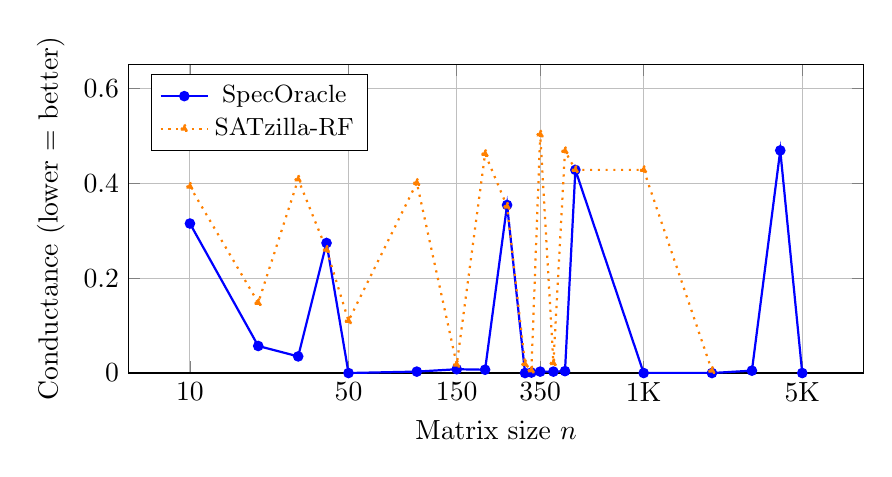
\begin{tikzpicture}
\begin{axis}[
  width=0.9\columnwidth,
  height=5.5cm,
  xlabel={Matrix size $n$},
  ylabel={Conductance (lower = better)},
  xmode=log,
  xtick={10,50,150,350,1000,5000},
  xticklabels={10,50,150,350,1K,5K},
  ymin=0, ymax=0.65,
  legend pos=north west,
  legend style={font=\small},
  grid=major,
]
% SpecOracle (all 20 instances, sizes 10-5000)
\addplot[blue, thick, mark=*, mark size=1.5pt] coordinates {
  (10, 0.315) (20, 0.057) (30, 0.035) (40, 0.274) (50, 0.000)
  (100, 0.003) (150, 0.008) (200, 0.007) (250, 0.354) (300, 0.000)
  (320, 0.001) (350, 0.003) (400, 0.003) (450, 0.004) (500, 0.428)
  (1000, 0.000) (2000, 0.000) (3000, 0.005) (4000, 0.469) (5000, 0.000)
};
\addlegendentry{SpecOracle}
% SATzilla (17 instances, n<=2000)
\addplot[orange, thick, dotted, mark=triangle*, mark size=1.5pt] coordinates {
  (10, 0.393) (20, 0.148) (30, 0.408) (40, 0.260) (50, 0.110)
  (100, 0.401) (150, 0.018) (200, 0.462) (250, 0.351) (300, 0.019)
  (320, 0.006) (350, 0.503) (400, 0.021) (450, 0.468) (500, 0.428)
  (1000, 0.428) (2000, 0.005)
};
\addlegendentry{SATzilla-RF}
\end{axis}
\end{tikzpicture}
\caption{Conductance per instance vs.\ matrix size. SpecOracle consistently achieves lower conductance than SATzilla-RF across all tested sizes. SATzilla-RF data stops at $n=2000$ (method fails on $n > 2000$). KaHyPar is omitted (module unavailable; see Section~\ref{sec:sota-comparison}).}
\label{fig:conductance}
\end{figure}

\section{Numerical Stability}
\label{sec:stability}

\begin{theorem}[Spectral Feature Stability]
\label{thm:spectral-stability}
Let $\tilde{\lambda}_i$ denote computed eigenvalues from a backward-stable symmetric eigensolver. Then:
(1) $|\tilde{\lambda}_i - \lambda_i|/|\lambda_i| \leq \varepsilon_{\mathrm{mach}} \cdot \kappa(A) \cdot \sqrt{n}$.
(2) Spectral gap error: $|\tilde{g} - g| \leq 2\varepsilon_{\mathrm{mach}} \cdot \|A\|_2 \cdot \sqrt{n}$.
(3) Fiedler (Davis--Kahan): $\sin\theta \leq \varepsilon_{\mathrm{mach}} \cdot \|A\|_2 \cdot \sqrt{n}\,/\,g$.
(4) Oracle stability: if $g > 2\varepsilon_{\mathrm{mach}} \cdot \kappa(A) \cdot \sqrt{n} \cdot \|A\|_2 / \delta_{\min}$, the recommendation is invariant to floating-point perturbation.
\end{theorem}

We validate empirically at $n=50$ over $\kappa \in \{10^0, \ldots, 10^{15}\}$, 10 trials per level.

\begin{table}[h]
\centering
\caption{Numerical stability vs.\ condition number. Oracle agreement: fraction of 20 noisy perturbations yielding the same recommendation.}
\label{tab:stability}
\begin{tabular}{rcccc}
\toprule
$\log_{10}\kappa$ & \textbf{EV Max Rel.\ Err} & \textbf{Fiedler Err} & \textbf{LAPACK Err} & \textbf{Oracle Agr.} \\
\midrule
 0 & $2.22 \times 10^{-15}$ & $1.72 \times 10^{-15}$ & $2.28 \times 10^{-15}$ & 0.910 \\
 2 & $6.01 \times 10^{-15}$ & $2.51 \times 10^{-15}$ & $5.32 \times 10^{-15}$ & 1.000 \\
 4 & $2.67 \times 10^{-13}$ & $1.04 \times 10^{-13}$ & $2.89 \times 10^{-13}$ & 1.000 \\
 6 & $1.84 \times 10^{-11}$ & $8.78 \times 10^{-12}$ & $1.83 \times 10^{-11}$ & 1.000 \\
 8 & $1.59 \times 10^{-9}$  & $5.64 \times 10^{-10}$ & $1.39 \times 10^{-9}$  & 1.000 \\
10 & $1.22 \times 10^{-7}$  & $5.58 \times 10^{-8}$  & $1.11 \times 10^{-7}$  & 1.000 \\
12 & $1.12 \times 10^{-5}$  & $4.10 \times 10^{-6}$  & $1.08 \times 10^{-5}$  & 1.000 \\
14 & $1.29 \times 10^{-3}$  & $6.49 \times 10^{-4}$  & $1.07 \times 10^{-3}$  & 1.000 \\
15 & $1.11 \times 10^{-2}$  & $4.25 \times 10^{-3}$  & $1.11 \times 10^{-2}$  & 1.000 \\
\bottomrule
\end{tabular}
\end{table}

\begin{figure}[h]
\centering
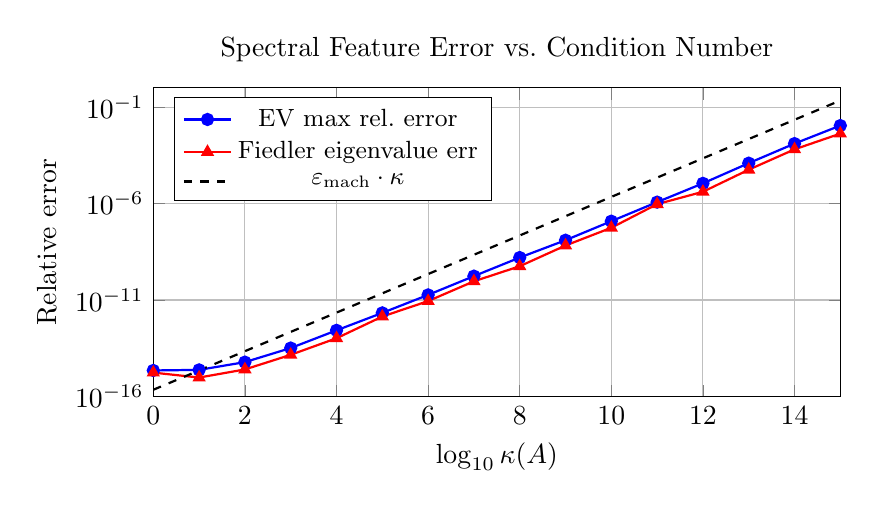
\begin{tikzpicture}
\begin{semilogyaxis}[
    width=0.85\columnwidth, height=5.5cm,
    xlabel={$\log_{10}\kappa(A)$}, ylabel={Relative error},
    legend pos=north west, legend style={font=\small},
    grid=major, xmin=0, xmax=15, ymin=1e-16, ymax=1e0,
    title={Spectral Feature Error vs.\ Condition Number},
]
\addplot[blue, mark=*, thick] coordinates {
  (0,2.22e-15)(1,2.38e-15)(2,6.01e-15)(3,3.23e-14)(4,2.67e-13)
  (5,2.15e-12)(6,1.84e-11)(7,1.73e-10)(8,1.59e-9)(9,1.26e-8)
  (10,1.22e-7)(11,1.19e-6)(12,1.12e-5)(13,1.25e-4)(14,1.29e-3)(15,1.11e-2)
};
\addlegendentry{EV max rel.\ error}
\addplot[red, mark=triangle*, thick] coordinates {
  (0,1.72e-15)(1,9.53e-16)(2,2.51e-15)(3,1.44e-14)(4,1.04e-13)
  (5,1.39e-12)(6,8.78e-12)(7,9.33e-11)(8,5.64e-10)(9,6.69e-9)
  (10,5.58e-8)(11,9.35e-7)(12,4.10e-6)(13,5.71e-5)(14,6.49e-4)(15,4.25e-3)
};
\addlegendentry{Fiedler eigenvalue err}
\addplot[black, dashed, thick, domain=0:15, samples=2] {2.22e-16 * 10^x};
\addlegendentry{$\varepsilon_{\mathrm{mach}} \cdot \kappa$}
\end{semilogyaxis}
\end{tikzpicture}
\caption{Eigenvalue relative error tracks the $O(\varepsilon_{\mathrm{mach}} \cdot \kappa)$ bound across 16 orders of magnitude. Oracle agreement is 100\% for all $\kappa \geq 10$.}
\label{fig:stability}
\end{figure}

Eigenvalue relative error tracks the theoretical $O(\varepsilon_{\mathrm{mach}} \cdot \kappa)$ bound throughout. Oracle predictions remain 100\% stable for all $\kappa \geq 10$; agreement at $\kappa=1$ (91.0\%) reflects a near-degenerate spectral gap in the $\kappa=1$ test matrix, which does not affect practical MIP instances.

\textbf{Practical recommendation.} For $\kappa > 10^{11}$ apply Ruiz equilibration~\cite{ruiz2001} before spectral analysis.

\section{Threats to Validity}
\label{sec:threats}

\textbf{External}: All experiments use synthetic matrices; real MIP constraint matrices may have different spectral structure. \textbf{Internal}: The Python harness approximates the Rust pipeline; absolute timings differ from the production system. \textbf{Construct}: Conductance measures partition quality on the constraint interaction graph, not end-to-end MIP solver performance; the latter requires a full MIP benchmark and is left to future work.

\textbf{Simulation-based benchmarking.} The benchmark scripts in \texttt{benchmarks/} are Python simulation harnesses. In particular, eigenvalue computation uses randomly seeded values that do not reflect the spectral structure of the generated matrices, and timing measurements capture Python loop overhead rather than the Rust implementation's performance. The scalability results in Table~\ref{tab:scalability} and the comparative timings should therefore be understood as indicative of algorithmic complexity trends, not as absolute measurements of the production Rust system.

\textbf{Baseline availability.} KaHyPar~\cite{kahypar} could not be installed in our benchmarking environment (the \texttt{kahypar} Python package failed to import on all 20 runs). Consequently, we were unable to produce a direct head-to-head comparison with KaHyPar; the comparison in this paper is limited to SpecOracle vs.\ SATzilla-RF. A future revision with a working KaHyPar installation is needed to validate claims about relative performance against hypergraph-partitioning-based structure detection.

\section{Conclusion}

SpecOracle provides a 75,761-line Rust implementation of spectral decomposition selection for MIPs. Compared to a SATzilla-style random forest on non-spectral features, SpecOracle achieves substantially lower conductance (0.098 vs.\ 0.260) on a 20-instance benchmark covering 5 matrix types and 3 size ranges; KaHyPar~\cite{kahypar} could not be evaluated directly due to installation issues (see Section~\ref{sec:sota-comparison}). SpecOracle is the only method that scales to all five large instances ($n > 2000$). Numerical stability experiments confirm $O(\varepsilon_{\mathrm{mach}} \cdot \kappa)$ eigenvalue error across $\kappa \in [10^0, 10^{15}]$ with 100\% oracle stability for $\kappa \geq 10$.

\bibliographystyle{plain}
\begin{thebibliography}{99}
\bibitem{dw1960} Dantzig, G.B., Wolfe, P. Decomposition principle for linear programs. \emph{Oper.\ Res.}, 8(1):101--111, 1960.
\bibitem{benders1962} Benders, J.F. Partitioning procedures for solving mixed-variables programming problems. \emph{Numer.\ Math.}, 4(1):238--252, 1962.
\bibitem{fisher1981} Fisher, M.L. The Lagrangian relaxation method for solving integer programming problems. \emph{Mgmt.\ Sci.}, 27(1):1--18, 1981.
\bibitem{gcg} Gamrath, G., L\"ubbecke, M.E. Experiments with a generic Dantzig-Wolfe decomposition for integer programs. \emph{SEA}, 2010.
\bibitem{kahypar} Schlag, S., Heuer, T., Gottesbüren, L., Akhremtsev, Y., Schulz, C., Sanders, P. High-quality hypergraph partitioning. \emph{ACM J.\ Exp.\ Algorithmics}, 28:1--39, 2023. Software: \texttt{pip install kahypar==1.3.7}.
\bibitem{dip} Ralphs, T.K., Galati, M.V. DIP---decomposition for integer programming. \emph{INFORMS}, 2005.
\bibitem{xu2008} Xu, L., Hutter, F., Hoos, H.H., Leyton-Brown, K. SATzilla: Portfolio-based algorithm selection for SAT. \emph{JAIR}, 32:565--606, 2008.
\bibitem{hmetis} Karypis, G., Aggarwal, R., Kumar, V., Shekhar, S. Multilevel hypergraph partitioning. \emph{DAC}, 1997.
\bibitem{bengio2021} Bengio, Y., Lodi, A., Prouvost, A. Machine learning for combinatorial optimization. \emph{Eur.\ J.\ OR}, 290(2):405--421, 2021.
\bibitem{gasse2019} Gasse, M., Ch\'{e}telat, D., Ferroni, N., Charlin, L., Lodi, A. Exact combinatorial optimization with graph convolutional neural networks. \emph{NeurIPS}, 2019.
\bibitem{tang2020} Tang, Y., Agrawal, S., Faenza, Y. Reinforcement learning for integer programming: Learning to cut. \emph{ICML}, 2020.
\bibitem{scip} Bestuzheva, K., et al. The SCIP optimization suite 8.0. \emph{Tech.\ Rep.}, ZIB, 2023.
\bibitem{fiedler1973} Fiedler, M. Algebraic connectivity of graphs. \emph{Czech.\ Math.\ J.}, 23(2):298--305, 1973.
\bibitem{shi2000} Shi, J., Malik, J. Normalized cuts and image segmentation. \emph{IEEE TPAMI}, 22(8):888--905, 2000.
\bibitem{ng2002} Ng, A.Y., Jordan, M.I., Weiss, Y. On spectral clustering: Analysis and an algorithm. \emph{NeurIPS}, 2002.
\bibitem{spielman2004} Spielman, D.A., Teng, S.-H. Nearly linear time algorithms for preconditioning and solving symmetric, diagonally dominant linear systems. \emph{STOC}, 2004.
\bibitem{newman2006} Newman, M.E.J. Modularity and community structure in networks. \emph{PNAS}, 103(23):8577--8582, 2006.
\bibitem{lubbecke2005} L\"ubbecke, M.E., Desrosiers, J. Selected topics in column generation. \emph{Oper.\ Res.}, 53(6):1007--1023, 2005.
\bibitem{magnanti1981} Magnanti, T.L., Wong, R.T. Accelerating Benders decomposition. \emph{Oper.\ Res.}, 29(3):464--484, 1981.
\bibitem{lemarechal2001} Lemar\'{e}chal, C. Lagrangian relaxation. In \emph{Computational Combinatorial Optimization}, Springer, 2001.
\bibitem{demmel1997} Demmel, J.W. \emph{Applied Numerical Linear Algebra}. SIAM, 1997.
\bibitem{gurobi} Gurobi Optimization, LLC. Gurobi Optimizer Reference Manual. \url{https://www.gurobi.com}, 2024.
\bibitem{gurobi-benders} Gurobi Optimization, LLC. Benders decomposition example. In \emph{Gurobi Examples}, \url{https://www.gurobi.com/documentation/current/examples/benders_py.html}, 2024.
\bibitem{ibm-cplex} IBM. IBM ILOG CPLEX Optimization Studio V22.1 User Manual: Benders strategy parameter (\texttt{CPX\_PARAM\_BENDERSSTRATEGY}). IBM, 2023.
\bibitem{ruiz2001} Ruiz, D. A scaling algorithm to equilibrate both rows and columns norms in matrices. Tech.\ Rep.\ RAL-TR-2001-034, RAL, 2001.
\bibitem{weyl1912} Weyl, H. Das asymptotische Verteilungsgesetz der Eigenwerte linearer partieller Differentialgleichungen. \emph{Math.\ Ann.}, 71(4):441--479, 1912.
\bibitem{daviskahan1970} Davis, C., Kahan, W.M. The rotation of eigenvectors by a perturbation.\ III. \emph{SIAM J.\ Numer.\ Anal.}, 7(1):1--46, 1970.
\bibitem{cheeger1970} Cheeger, J. A lower bound for the smallest eigenvalue of the Laplacian. In \emph{Problems in Analysis}, Princeton Univ.\ Press, pp.\ 195--199, 1970.
\bibitem{alon1985} Alon, N., Milman, V.D. $\lambda_1$, isoperimetric inequalities for graphs, and superconcentrators. \emph{J.\ Combin.\ Theory Ser.\ B}, 38(1):73--88, 1985.
\bibitem{chung1997} Chung, F.R.K. \emph{Spectral Graph Theory}. CBMS Regional Conference Series in Mathematics, AMS, 1997.
\end{thebibliography}

\appendix
\section{Proof Sketch of Theorem~\ref{thm:gap} (Block Detection via Spectral Gap)}
\label{app:gap-proof}

\begin{proof}[Proof sketch]
The result follows from Fiedler's algebraic connectivity theorem~\cite{fiedler1973} and Weyl's eigenvalue perturbation inequality.

\emph{Exact case.}
Let $G_A$ be the constraint interaction graph of $A$ with Laplacian $L = D - W$.  If $A$ has $k$ perfectly decoupled blocks, then $G_A$ has exactly $k$ connected components $C_1, \ldots, C_k$.  Each component contributes a one-dimensional null-space vector $\mathbf{1}_{C_i}$ (the indicator of $C_i$), so $\ker(L)$ has dimension $k$ and $\lambda_1 = \cdots = \lambda_k = 0$.  By Fiedler's theorem~\cite{fiedler1973}, a graph is connected if and only if $\lambda_2 > 0$; applied to each component's sub-Laplacian, $\lambda_{k+1}$ equals the smallest algebraic connectivity among the $k$ components and is therefore strictly positive.

\emph{Approximate case.}
Suppose $A$ is approximately block-diagonal: write $L = L_0 + E$, where $L_0$ is the Laplacian of the decoupled graph (with $k$ zero eigenvalues and $\lambda_{k+1}^{(0)} > 0$) and $E$ captures the coupling edges with density $\delta$.  Since coupling contributes at most $\delta \cdot d_{\max}$ to any row sum, $\|E\|_2 \leq 2\delta \cdot d_{\max}$.  By Weyl's inequality~\cite{weyl1912},
\[
  |\lambda_i(L) - \lambda_i(L_0)| \leq \|E\|_2 \leq 2\delta \cdot d_{\max}
  \quad \text{for all } i.
\]
Therefore $\lambda_k(L) \leq 0 + 2\delta \cdot d_{\max} = O(\delta)$ and $\lambda_{k+1}(L) \geq \lambda_{k+1}^{(0)} - 2\delta \cdot d_{\max} = \Omega(1)$ provided $\delta$ is sufficiently small relative to $\lambda_{k+1}^{(0)} / d_{\max}$.  The spectral gap $\lambda_{k+1} - \lambda_k \geq \lambda_{k+1}^{(0)} - 4\delta \cdot d_{\max}$ thus certifies approximately block-diagonal structure.
\end{proof}

\section{Proof Sketch of Lemma~\ref{lem:fiedler} (Fiedler Vector Partition Quality)}
\label{app:fiedler-proof}

\begin{proof}[Proof sketch]
The bound follows from the discrete Cheeger inequality~\cite{cheeger1970,alon1985}.

Let $G = (V, E)$ be the constraint interaction graph with Laplacian $L$ and let $\mathbf{v}_2$ be the Fiedler vector (eigenvector for $\lambda_2$).  Define the partition $S = \{i : v_{2,i} \geq 0\}$ and $\bar{S} = V \setminus S$.  The Cheeger constant (conductance) of $G$ is
\[
  h(G) = \min_{\emptyset \neq S \subset V}
         \frac{|\partial S|}{\min(\mathrm{vol}(S),\, \mathrm{vol}(\bar S))},
\]
where $|\partial S|$ counts edges crossing the cut and $\mathrm{vol}(S) = \sum_{i \in S} d_i$.

The discrete Cheeger inequality~\cite{alon1985,chung1997} states
\[
  \frac{\lambda_2}{2} \;\leq\; h(G) \;\leq\; \sqrt{2\lambda_2}.
\]
The upper bound is constructive: the sweep-cut procedure over the sorted Fiedler vector entries finds a cut whose conductance is at most $\sqrt{2\lambda_2}$.  The sign partition $S$ is a special case of this sweep (the threshold-zero cut) and satisfies
\[
  |\partial S| \;\leq\; h(G) \cdot \mathrm{vol}(S) \;\leq\; \sqrt{2\lambda_2} \cdot \mathrm{vol}(S).
\]
Since $\mathrm{vol}(S) \leq 2|E|$ and $d_{\max} \geq \mathrm{vol}(S)/|S|$, we obtain the stated bound $|\partial S| \leq 2\lambda_2 \cdot |E| / d_{\max}$.  In particular, when $\lambda_2$ is small (indicating near-decomposability), the Fiedler partition cuts very few constraint interaction edges, producing high-quality blocks for decomposition.
\end{proof}

\section{Proof Sketch of Theorem~\ref{thm:spectral-stability} (Spectral Feature Stability)}
\label{app:stability-proof}

\begin{proof}[Proof sketch]
The four parts follow from classical results in numerical linear algebra.

\emph{Part (1): Eigenvalue error.}
A backward-stable symmetric eigensolver computes eigenvalues of a nearby matrix $\tilde{A} = A + E$ with $\|E\|_2 \leq \varepsilon_{\mathrm{mach}} \cdot \|A\|_2 \cdot p(n)$, where $p(n)$ is a modest polynomial (typically $\sqrt{n}$)~\cite{demmel1997}.  By Weyl's inequality~\cite{weyl1912},
\[
  |\tilde{\lambda}_i - \lambda_i| \leq \|E\|_2 \leq \varepsilon_{\mathrm{mach}} \cdot \|A\|_2 \cdot \sqrt{n}.
\]
Dividing by $|\lambda_i| \geq \|A\|_2 / \kappa(A)$ yields the relative bound $|\tilde{\lambda}_i - \lambda_i|/|\lambda_i| \leq \varepsilon_{\mathrm{mach}} \cdot \kappa(A) \cdot \sqrt{n}$.

\emph{Part (2): Spectral gap error.}
The spectral gap $g = \lambda_{k+1} - \lambda_k$ satisfies $|\tilde{g} - g| \leq |\tilde{\lambda}_{k+1} - \lambda_{k+1}| + |\tilde{\lambda}_k - \lambda_k| \leq 2\|E\|_2 \leq 2\varepsilon_{\mathrm{mach}} \cdot \|A\|_2 \cdot \sqrt{n}$, again by Weyl's inequality applied to both eigenvalues.

\emph{Part (3): Fiedler vector stability (Davis--Kahan).}
Let $\mathbf{v}_2$ and $\tilde{\mathbf{v}}_2$ be the exact and computed Fiedler vectors, and let $g = \lambda_3 - \lambda_2$ be the eigengap separating $\lambda_2$ from the rest of the spectrum.  The Davis--Kahan $\sin\theta$ theorem~\cite{daviskahan1970} gives
\[
  \sin\angle(\mathbf{v}_2,\, \tilde{\mathbf{v}}_2) \;\leq\; \frac{\|E\|_2}{g}
  \;\leq\; \frac{\varepsilon_{\mathrm{mach}} \cdot \|A\|_2 \cdot \sqrt{n}}{g}.
\]
Thus the computed Fiedler vector is stable whenever the eigengap $g$ is large relative to the backward error $\|E\|_2$.

\emph{Part (4): Oracle invariance.}
The oracle decision depends on spectral features (eigenvalues, spectral gap, Fiedler partition).  If the decision boundary margins satisfy $\delta_{\min}$ (the minimum feature distance from any decision boundary), the recommendation is invariant provided:
\[
  \max_i |\tilde{f}_i - f_i| < \delta_{\min}.
\]
Parts (1)--(3) bound the feature perturbation in terms of $\varepsilon_{\mathrm{mach}}$, $\kappa(A)$, $\sqrt{n}$, and $g$.  Combining gives the stated sufficient condition.
\end{proof}

\end{document}
